\section{Einführung in gewöhnliche Differentialgleichungen}

\section{Differentialgleichungen}

\begin{definition}{Differentialgleichung}
  \(n\)-ter Ordnung ist ein Gleichung von der Form:
      \[F(x,y,y',y'',\ldots,y^{(n)})=0\]
  \begin{itemize}
    \item Eine Differentialgleichung 
      für eine gesuchte Funktion \(y=y(x)\), in der Ableitungen von \(y(x)\) bis zur \(n\)-ten Ordnung auftreten.
    \item Falls die DGL nach \(y^{(n)}\) aufgelöst ist, nennt man sie explizit, ansonsten implizit.
      Oft können implizite DGL durch einfaches Umformen in explizite DGL umgewandelt werden.
  \end{itemize}
\end{definition}

\begin{definition}{Arten von DGL}
  \begin{itemize}
    \item \emph{Separierbar:} falls \(F(x,y)\) als Produkt eines \(x\)- und eines \(y\)-Anteils geschrieben
      werden kann, d.h. es hat die Form:
      \[y'=g(x)\cdot h(y)\]
    \item \emph{Autonom:} falls \(F(x,y)\) nur von \(y\) abhängt, d.h. es hat die Form:
      \[y'=f(y)\]
    \item \emph{Linear:} falls die Variabel welche abgeleitet wird, nur in der ersten Potenz vorkommt und nicht
      multipliziert miteinander oder mit der unabhängigen Variabel wird.
  \end{itemize}
\end{definition}

\begin{KR}{Lösen von Separierbaren DGL}
  \begin{center}
    DGL:
      $\frac{\mathrm{d}y}{\mathrm{d}x}=g(x)\cdot h(y)$\\
      \vspace{1mm}
      $\rightarrow$ Falls \(h(y_0)=0\), ist \(y=y_0\) eine Lösung der DGL.
  \end{center}
  \begin{itemize}
    \item Trennung aller \(x\)- und \(y\)-Terme:
    $\frac{1}{h(y)}\cdot \mathrm{d}y=g(x)\cdot \mathrm{d}x$
    \item Integration auf beiden Seiten:
    $\int{\frac{1}{h(y)}\mathrm{d}y}=\int{g(x)\mathrm{d}x}$
    \end{itemize}
  Auflösen nach \(y\), Anfangsbedingungen einsetzen:
      \[\int_{y_0}^{y}{\frac{1}{h(s)}\mathrm{d}s}=\int_{x_0}^{x}{g(t)\mathrm{d}t}\]
\end{KR}

\begin{definition}{Homogenität von DGL}
  \begin{itemize}
    \item Homogene DGL: \(F(x,y,y',y'',\ldots,y^{(n)})=0\)
    \item Inhomogene DGL: \(F(x,y,y',y'',\ldots,y^{(n)})=g(x)\)
    \begin{itemize}
      \item \(g(x)\) ist die Störfunktion
    \end{itemize}
  \end{itemize}
\end{definition}

\begin{formula}{Allgemeine Lösung der inhomogenen DGL}
  $y'+f(x)y=g(x)$
      ist gegeben durch:
      \[y=e^{-F(x)}\cdot \int{g(x)e^{F(x)}\mathrm{d}x}\]
      wobei \(F(x)\) eine Stammfunktion von \(f(x)\) ist.

\end{formula}

\begin{definition}{Anfangswertproblem} DGL mit Anfangsbedingung\\
  Anfangswertproblem \(n\)-ter Ordnung:
      \[\left\{\begin{tabular}{rcl}
	  \( F(x,y,y',y'',\ldots,y^{(n)})\)&\(=\)&\(0,\;(x,y,\ldots,y^{(n)})\in \Omega\)\\
	  \(y(x_0)\)&\(=\)&\(y_0\)\\
	  \(y'(x_0)\)&\(=\)&\(y_1\)\\
		\(\) &\(\vdots\)&\(\)\\
	 \( y^{n-1}(x_0)\)&\(=\)&\( y_{n-1}\)
      \end{tabular}\right.\]
      Anfangswertproblem für explizite DGL 1. Ordnung:
      \[\left\{\begin{tabular}{rcl}
	  \(y'\)&\(=\)&\(G(x,y),\quad (x,y,y')\in \Omega\subseteq\mathbb{R}\times\mathbb{R}^2\)\\
	  \(y(x_0)\)&\(=\)&\(y_0\)
      \end{tabular}\right.\]
  \begin{itemize}
    \item Allgemeine Lösung: Menge aller Lösungen einer DGL
    \item Spezielle/partikuläre Lösung: Lösung eines Anfangswertproblems
  \end{itemize}
\end{definition}

\begin{KR}{Lösung von Anfangswertproblemen mit seperiarbaren DGL}
  \begin{itemize}
    \item Sind \(g(x)\) und \(h(y)\) stetige Funktionen und \((x_0,y_0)\in \mathbb{R}^2\) mit \(h(y_0)\neq 0\), hat das
      Anfangswertproblem:
      \[\left\{\begin{tabular}{rcl}
	  \(y'\)&\(=\)&\(g(x)h(y)\)\\
	  \(y(x_0)\)&\(=\)&\(y_0\)\\
      \end{tabular}\right.\]
      genau eine Lösung. Sie kann gefunden werden, indem beide Seiten von 
      \[\int_{y_0}^{y}{\frac{1}{h(s)}\mathrm{d}s}=\int_{x_0}^{x}{g(t)\mathrm{d}t}\]
      berechnet werden und nach \(y\) aufgelöst werden.
  \end{itemize}
\end{KR}

\paragraph{Richtungsfeder}
\begin{definition}{Richtungsfeld} geometrisches Verständnis von expliziten DGL 1. Ordnung, d.h. DGL der Form:
  $y'=f(x,y)$
  %\vspace{3mm}  \\
  \begin{minipage}{0.45\linewidth}
    \begin{center}
    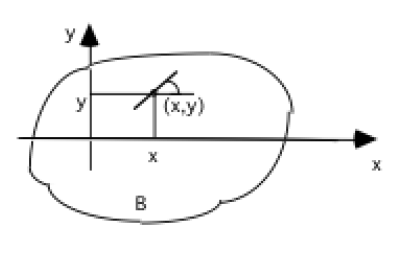
\includegraphics[width=0.8\linewidth]{Richtungsfeld.png}
    \end{center}
  \end{minipage}
  \hspace{3mm}
  \begin{minipage}{0.45\linewidth}
    \begin{center}
    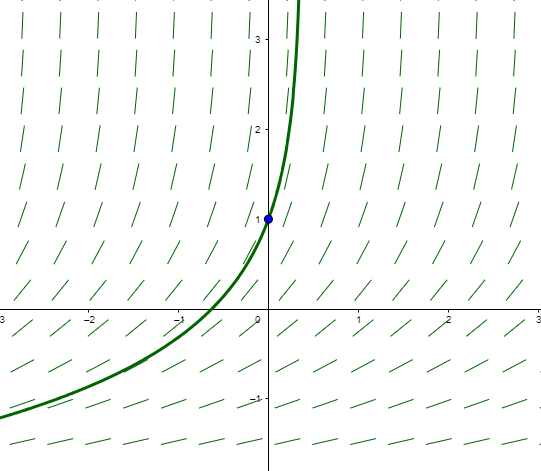
\includegraphics[width=0.8\linewidth]{RichtungsfeldKurve.png}
    \end{center}
  \end{minipage}

  \begin{minipage}{0.45\linewidth}
    \(f(x,y)\) gibt also die Steigung der Lösungskurve am Punkt \((x,y)\) an
  \end{minipage}
  \hspace{3mm}
  \begin{minipage}{0.45\linewidth}
    Jeder Punkt ist somit die Tangente einer spezifischen Lösungskurve
  \end{minipage}
\end{definition}

\begin{definition}{Richtungsfelder von Speziellen DGL}\\
  \begin{minipage}{0.58\linewidth}
    Unbestimmtes Integral: \(y'=f(x)\)\\ das Richtungsfeld ist unabhängig von \(y\) die verschiedenen Lösungen
      unterscheiden sich nur durch eine verschiebung in \(y\)-Richtung durch die Konstante \(C\).
  \end{minipage}
  \begin{minipage}{0.4\linewidth}
    \begin{center}
      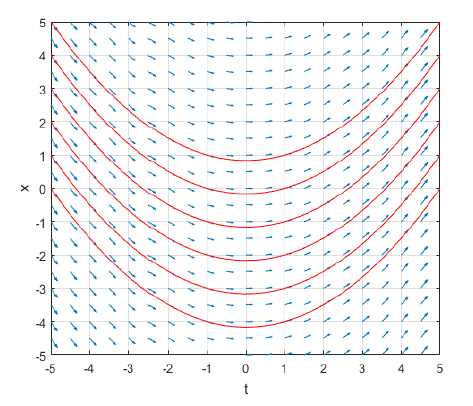
\includegraphics[width=1\linewidth]{UnbestimmtesIntegral.png}
      \end{center}
  \end{minipage}
  \begin{minipage}{0.58\linewidth}
    Autonome DGL:\(y'=f(y)\)\\ das Richtungsfeld ist unabhängig von \(x\) die Verschiedenen Lösungen gehen durch
    Verschiebung in \(x\)-Richtung in einander über.
  \end{minipage}
  \begin{minipage}{0.4\linewidth}
    \begin{center}
      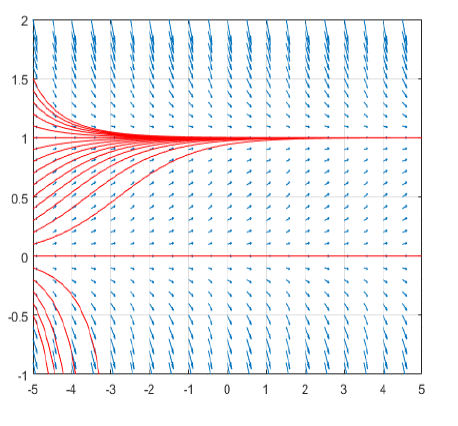
\includegraphics[width=1\linewidth]{AutonomeDGL.png}
      \end{center}
  \end{minipage}
\end{definition}






\paragraph{Numerische Verfahren}
\begin{definition}{Eulerverfahren}
  Gleichung einer beliebigen Geraden mit Steigung \(m\) am Punkt \((x_k,y_k)\):
      \[y=y_k+m\cdot(x-x_k)\]
    \begin{minipage}{0.5\linewidth}
      DGL am Punkt \((x_k,y_k)\):
      \[y=y_k+f(x_k,y_k)\cdot (x-x_k)\]
    \end{minipage}
    \begin{minipage}{0.45\linewidth}
      \begin{center}
        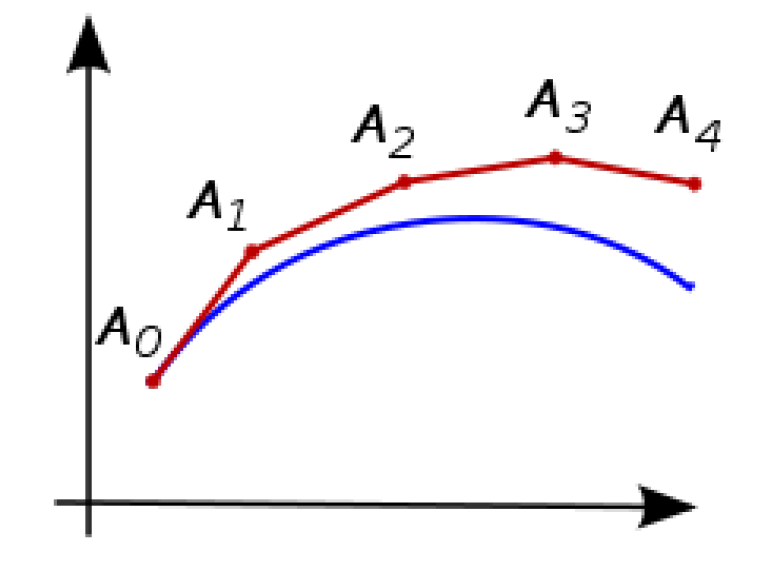
\includegraphics[width=0.7\linewidth]{Newtonverfahren.png}
        \end{center}
    \end{minipage}
  \begin{itemize}

    \item Für \(k=0 \text{ und } x=x_0\):
      \[\underbrace{y_1}_{\approx y(x_1)}=y_0+f(x_0,y_0)\cdot\underbrace{(x_1-x_0)}_{=h}\]
    \item Algorithmus für beliebige \(k\):
      \[\left\{\begin{tabular}{rcl}
	  \(x_k\)&\(=\)&\(x_0+k\cdot h\)\\
	  \(y_{k+1}\)&\(=\)&\(y_k+h\cdot f(x_k,y_k)\)
	\end{tabular}
      \right.\]
  \end{itemize}
  Problem: Die Steigung wird nur am linken Ende des Intervalls berücksichtigt!
    \\ $\Rightarrow$ Lösung: Verbesserte numerische Verfahren!
\end{definition}


\begin{definition}{Gewöhnliche Differentialgleichung n-ter Ordnung}\\
Eine Gleichung, in der Ableitungen einer unbekannten Funktion $y = y(x)$ bis zur $n$-ten Ordnung auftreten, heißt eine gewöhnliche Differentialgleichung $n$-ter Ordnung. Sie hat die explizite Form:
$$y^{(n)}(x) = f(x, y(x), y'(x), ..., y^{(n-1)}(x))$$

Gesucht sind die Lösungen $y = y(x)$ dieser Gleichung, wobei die Lösungen $y$ auf einem Intervall $[a,b]$ definiert sein sollen.

\textbf{Notationen für Ableitungen:}
$$\text{\textbf{Lagrange: }} y'(x), y''(x), y'''(x), y^{(4)}(x), ..., y^{(n)}(x)$$
$$\text{\textbf{Newton: }} \dot{y}(x), \ddot{y}(x), \dddot{y}(x), ...$$
$$\text{\textbf{Leibniz: }} \frac{dy}{dx}, \frac{d^2y}{dx^2}, \frac{d^3y}{dx^3}, ..., \frac{d^ny}{dx^n}$$
\end{definition}

\begin{definition}{Anfangswertproblem (AWP)}\\
Bei einem Anfangswertproblem für eine Differentialgleichung $n$-ter Ordnung werden der Lösungsfunktion $y = y(x)$ noch $n$ Werte vorgeschrieben:

\textbf{DGL 1. Ordnung:} \\
Gegeben ist $y'(x) = f(x, y(x))$ und der Anfangswert $y(x_0) = y_0$.
\vspace{2mm}\\
\textbf{DGL 2. Ordnung:} 
Gegeben ist $y''(x) = f(x, y(x), y'(x))$ und die Anfangswerte $y(x_0) = y_0$, $y'(x_0) = y_0'$.
\end{definition}

\begin{example2}{Beispiele aus den Naturwissenschaften}\\
\textbf{Aufgabe:} Klassifizieren Sie die folgenden DGL und geben Sie physikalische Interpretationen an.
\tcblower
\textbf{1. Radioaktiver Zerfall:}
$$\frac{dn}{dt} = -\lambda n$$
DGL 1. Ordnung, Lösung: $n(t) = n_0 e^{-\lambda t}$
\vspace{2mm}\\
\textbf{2. Freier Fall:}
$$\ddot{s}(t) = -g$$
DGL 2. Ordnung, Lösung: $s(t) = -\frac{1}{2}gt^2 + v_0 t + s_0$
\vspace{2mm}\\
\textbf{3. Harmonische Schwingung (Federpendel):}
$$m\ddot{x} = -cx \Rightarrow \ddot{x} + \frac{c}{m}x = 0$$
DGL 2. Ordnung, Lösung: $x(t) = A \sin(\omega_0 t + \varphi)$ mit $\omega_0 = \sqrt{\frac{c}{m}}$
\end{example2}

\raggedcolumns
\columnbreak

\subsection{Richtungsfelder}

\begin{concept}{Geometrische Interpretation}\\
Die DGL $y'(x) = f(x, y(x))$ gibt uns einen Zusammenhang zwischen der Steigung $y'(x)$ der gesuchten Funktion und dem Punkt $(x, y(x))$.

Im Richtungsfeld wird an jedem Punkt $(x,y)$ die Steigung $y'(x) = f(x,y)$ durch einen kleinen Pfeil dargestellt. Die Lösungskurven verlaufen stets tangential zu diesen Pfeilen.
\end{concept}

\begin{KR}{Richtungsfeld zeichnen und interpretieren}
\paragraph{Schritt 1: Steigungen berechnen}
Für eine gegebene DGL $y' = f(x,y)$ berechne für verschiedene Punkte $(x_i, y_j)$ die Steigung $f(x_i, y_j)$.

\paragraph{Schritt 2: Richtungspfeile einzeichnen}
Zeichne an jedem Punkt $(x_i, y_j)$ einen kleinen Pfeil mit der Steigung $f(x_i, y_j)$.

\paragraph{Schritt 3: Lösungskurven folgen}
Von einem Anfangspunkt $(x_0, y_0)$ ausgehend folge den Richtungspfeilen, um die Lösungskurve zu approximieren.

\paragraph{Schritt 4: Python-Implementierung}
Verwende \texttt{numpy.meshgrid()} und \texttt{pyplot.quiver()} zur automatischen Darstellung.
\end{KR}

\begin{example2}{Richtungsfeld interpretieren}\\
\textbf{Aufgabe:} Zeichnen Sie das Richtungsfeld für $\frac{dy}{dt} = -\frac{1}{2} \cdot y \cdot t^2$ und bestimmen Sie die Lösungskurve für $y(0) = 3$.
\tcblower
\textbf{Lösung:}

\textbf{Steigungen an ausgewählten Punkten:}
\begin{center}
\begin{tabular}{|c|c|c|c|c|}
\hline
$\frac{dy}{dt}$ & $t=0$ & $t=1$ & $t=2$ & $t=3$ \\
\hline
$y=0$ & 0 & 0 & 0 & 0 \\
\hline
$y=1$ & 0 & -0.5 & -2 & -4.5 \\
\hline
$y=2$ & 0 & -1 & -4 & -9 \\
\hline
$y=3$ & 0 & -1.5 & -6 & -13.5 \\
\hline
\end{tabular}
\end{center}

Die Lösungskurve für $y(0) = 3$ folgt den Richtungspfeilen und zeigt exponentiellen Abfall für $t > 0$.
\end{example2}

\raggedcolumns
\pagebreak

\subsection{Numerische Lösungsverfahren}

\subsubsection{Das Euler-Verfahren}

\begin{theorem}{Klassisches Euler-Verfahren}\\
Gegeben sei das AWP $y' = f(x,y)$ mit $y(a) = y_0$ auf dem Intervall $[a,b]$.

Das Euler-Verfahren mit Schrittweite $h = \frac{b-a}{n}$ lautet:
$$x_{i+1} = x_i + h$$
$$y_{i+1} = y_i + h \cdot f(x_i, y_i)$$

wobei $x_0 = a$, $x_i = a + ih$ für $i = 0, ..., n-1$ und $y_0$ der gegebene Anfangswert ist.
\end{theorem}

\begin{concept}{Idee des Euler-Verfahrens}\\
Das Euler-Verfahren folgt der Tangente im Punkt $(x_i, y_i)$ mit der Steigung $f(x_i, y_i)$ um die Schrittweite $h$. Es ist das einfachste Einschrittverfahren mit Konvergenzordnung $p = 1$.
\end{concept}

\begin{KR}{Euler-Verfahren anwenden}
\paragraph{Schritt 1: Parameter bestimmen}
Gegeben: AWP $y' = f(x,y)$, $y(a) = y_0$, Intervall $[a,b]$, Anzahl Schritte $n$
Berechne: $h = \frac{b-a}{n}$

\paragraph{Schritt 2: Startwerte setzen}
$x_0 = a$, $y_0 = $ gegebener Anfangswert

\paragraph{Schritt 3: Iteration}
Für $i = 0, 1, ..., n-1$:
\begin{itemize}
    \item Berechne $f(x_i, y_i)$
    \item Setze $x_{i+1} = x_i + h$
    \item Setze $y_{i+1} = y_i + h \cdot f(x_i, y_i)$
\end{itemize}

\paragraph{Schritt 4: Lösung interpretieren}
Die Punkte $(x_i, y_i)$ approximieren die Lösung $y(x)$ an den Stützstellen.
\end{KR}

\begin{example2}{Euler-Verfahren berechnen}\\
\textbf{Aufgabe:} Lösen Sie $\frac{dy}{dx} = \frac{x^2}{y}$ mit $y(0) = 2$ auf dem Intervall $[0, 1.4]$ mit $h = 0.7$ (Euler-Verfahren).
\tcblower
\textbf{Lösung:}

\textbf{Parameter:} $n = 2$, $h = 0.7$, $f(x,y) = \frac{x^2}{y}$

\textbf{Iteration:}
\begin{itemize}
    \item $i = 0$: $x_0 = 0$, $y_0 = 2$
    \item $f(0, 2) = \frac{0^2}{2} = 0$
    \item $x_1 = 0 + 0.7 = 0.7$, $y_1 = 2 + 0.7 \cdot 0 = 2$
\end{itemize}

\begin{itemize}
    \item $i = 1$: $x_1 = 0.7$, $y_1 = 2$
    \item $f(0.7, 2) = \frac{0.7^2}{2} = 0.245$
    \item $x_2 = 0.7 + 0.7 = 1.4$, $y_2 = 2 + 0.7 \cdot 0.245 = 2.1715$
\end{itemize}

\textbf{Exakte Lösung:} $y(x) = \sqrt{\frac{2x^3}{3} + 4}$
$y(1.4) = \sqrt{\frac{2 \cdot 1.4^3}{3} + 4} = 2.253$

\textbf{Absoluter Fehler:} $|2.253 - 2.1715| = 0.0815$
\end{example2}

\subsubsection{Verbesserte Euler-Verfahren}

\begin{theorem}{Mittelpunkt-Verfahren}\\
Das Mittelpunkt-Verfahren berechnet die Steigung in der Mitte des Intervalls:
$$x_{h/2} = x_i + \frac{h}{2}$$
$$y_{h/2} = y_i + \frac{h}{2} \cdot f(x_i, y_i)$$
$$x_{i+1} = x_i + h$$
$$y_{i+1} = y_i + h \cdot f(x_{h/2}, y_{h/2})$$

Konvergenzordnung: $p = 2$
\end{theorem}

\begin{corollary}{Modifiziertes Euler-Verfahren (Heun-Verfahren)}\\
Das modifizierte Euler-Verfahren verwendet den Durchschnitt zweier Steigungen:
$$k_1 = f(x_i, y_i)$$
$$k_2 = f(x_i + h, y_i + h \cdot k_1)$$
$$x_{i+1} = x_i + h$$
$$y_{i+1} = y_i + h \cdot \frac{k_1 + k_2}{2}$$

Konvergenzordnung: $p = 2$
\end{corollary}

\begin{example2}{Vergleich der Euler-Verfahren}\\
\textbf{Aufgabe:} Lösen Sie das AWP aus dem vorigen Beispiel mit Mittelpunkt- und modifiziertem Euler-Verfahren. Vergleichen Sie die Genauigkeit.
\tcblower
\textbf{Mittelpunkt-Verfahren:}
\begin{itemize}
    \item $x_{1/2} = 0.35$, $y_{1/2} = 2$, $f(0.35, 2) = 0.061$
    \item $y_1 = 2 + 0.7 \cdot 0.061 = 2.043$
    \item $x_{3/2} = 1.05$, $y_{3/2} = 2.128$, $f(1.05, 2.128) = 0.518$
    \item $y_2 = 2.043 + 0.7 \cdot 0.518 = 2.406$
\end{itemize}
\vspace{2mm}
\textbf{Modifiziertes Euler-Verfahren:}
\begin{itemize}
    \item $k_1 = 0$, $k_2 = f(0.7, 2) = 0.245$
    \item $y_1 = 2 + 0.7 \cdot \frac{0 + 0.245}{2} = 2.086$
    \item $k_1 = 0.245$, $k_2 = f(1.4, 2.257) = 0.866$
    \item $y_2 = 2.086 + 0.7 \cdot \frac{0.245 + 0.866}{2} = 2.475$
\end{itemize}
\vspace{2mm}
\textbf{Fehlervergleich bei $x = 1.4$:}
\begin{itemize}
    \item Exakt: $y(1.4) = 2.253$
    \item Euler: $|2.253 - 2.172| = 0.081$
    \item Mittelpunkt: $|2.253 - 2.406| = 0.153$
    \item Modifiziert: $|2.253 - 2.475| = 0.222$
\end{itemize}
\end{example2}

\subsubsection{Runge-Kutta Verfahren}

\begin{theorem}{Klassisches vierstufiges Runge-Kutta Verfahren}\\
Das klassische Runge-Kutta Verfahren verwendet vier Steigungen und hat Konvergenzordnung $p = 4$:
\vspace{-2mm}\\
$$k_1 = f(x_i, y_i), \quad
k_2 = f(x_i + \frac{h}{2}, y_i + \frac{h}{2} k_1)$$
$$k_3 = f(x_i + \frac{h}{2}, y_i + \frac{h}{2} k_2), \quad
k_4 = f(x_i + h, y_i + h k_3)$$
$$x_{i+1} = x_i + h, \quad
y_{i+1} = y_i + h \cdot \frac{1}{6}(k_1 + 2k_2 + 2k_3 + k_4)$$
\end{theorem}

\begin{concept}{Butcher-Schema}
    Runge-Kutta Verfahren werden durch Butcher-Schemata charakterisiert:

    \begin{minipage}{0.45\textwidth}
        \begin{center}
        \begin{tabular}{c|cccc}
        0 & & & & \\
        $\frac{1}{2}$ & $\frac{1}{2}$ & & & \\
        $\frac{1}{2}$ & 0 & $\frac{1}{2}$ & & \\
        1 & 0 & 0 & 1 & \\
        \hline
        & $\frac{1}{6}$ & $\frac{1}{3}$ & $\frac{1}{3}$ & $\frac{1}{6}$
        \end{tabular}
        \end{center}
    \end{minipage}
    \begin{minipage}{0.54\textwidth}
        \textbf{Interpretation:} Die erste Spalte gibt die Stufen $c_i$, 
        die zweite Spalte die Koeffizienten $a_{ij}$ für die Steigungen $k_j$ und die letzte Zeile die Gewichtung der Steigungen für die nächste Iteration an.
    \end{minipage}

\end{concept}

\begin{KR}{Runge-Kutta Verfahren anwenden}
\paragraph{Schritt 1: Steigungen berechnen}
\vspace{-2mm}
$$k_1 = f(x_i, y_i), \quad
k_2 = f(x_i + \frac{h}{2}, y_i + \frac{h}{2} k_1)$$
$$k_3 = f(x_i + \frac{h}{2}, y_i + \frac{h}{2} k_2), \quad
k_4 = f(x_i + h, y_i + h k_3)$$

\paragraph{Schritt 2: Gewichtetes Mittel bilden}
\vspace{-2mm}
$$\text{Steigung} = \frac{1}{6}(k_1 + 2k_2 + 2k_3 + k_4)$$

\paragraph{Schritt 3: Nächsten Punkt berechnen}
\vspace{-2mm}
$$x_{i+1} = x_i + h, \quad
y_{i+1} = y_i + h \cdot \text{Steigung}$$

\paragraph{Schritt 4: Iteration fortsetzen}
Wiederhole bis zum Ende des Intervalls.
\end{KR}

\begin{example2}{Runge-Kutta vs. andere Verfahren}\\
\textbf{Aufgabe:} Lösen Sie $y' = 1 - \frac{y}{t}$ mit $y(1) = 5$ für $t \in [1,6]$ mit $h = 0.01$ und vergleichen Sie mit der exakten Lösung $y(t) = \frac{t^2 + 9}{2t}$.

\begin{lstlisting}[language=Python, style=basesmol]
def runge_kutta_4(f, a, b, n, y0):
    h = (b - a) / n
    x = a
    y = y0
    
    for i in range(n):
        k1 = f(x, y)
        k2 = f(x + h/2, y + h/2 * k1)
        k3 = f(x + h/2, y + h/2 * k2)
        k4 = f(x + h, y + h * k3)
        
        x += h
        y += h * (k1 + 2*k2 + 2*k3 + k4) / 6
        
    return x, y
\end{lstlisting}

\textbf{Fehlervergleich bei $t = 6$:}
\begin{itemize}
    \item Exakt: $y(6) = 3.25$
    \item Euler: Fehler $\approx 0.1$
    \item Runge-Kutta: Fehler $\approx 10^{-6}$
\end{itemize}
\end{example2}

\subsection{Systeme von Differentialgleichungen}

\begin{concept}{DGL höherer Ordnung $\rightarrow$ System 1. Ordnung}\\
Jede DGL $n$-ter Ordnung kann in ein System von $n$ DGL 1. Ordnung umgewandelt werden durch Einführung von Hilfsvariablen für die Ableitungen.
\end{concept}

\begin{KR}{DGL höherer Ordnung auf System 1. Ordnung zurückführen}
\paragraph{Schritt 1: Nach höchster Ableitung auflösen}
Bringe die DGL in die Form $y^{(n)} = f(x, y, y', ..., y^{(n-1)})$.
\vspace{2mm}\\
\begin{minipage}{0.45\linewidth}
\paragraph{Schritt 2: Hilfsvariablen einführen}
\vspace{-3mm}
$$z_1(x) = y(x)$$
$$z_2(x) = y'(x)$$
$$z_3(x) = y''(x)$$
$$...$$
$$z_n(x) = y^{(n-1)}(x)$$
\end{minipage}
\hspace{2mm}
\begin{minipage}{0.5\linewidth}
\paragraph{Schritt 3: System aufstellen}
\vspace{-3mm}
$$z_1' = z_2$$
$$z_2' = z_3$$
$$...$$
$$z_{n-1}' = z_n$$
$$z_n' = f(x, z_1, z_2, ..., z_n)$$
\end{minipage}

\paragraph{Schritt 4: Vektorielle Schreibweise}
$\mathbf{z}' = \mathbf{f}(x, \mathbf{z})$ mit $\mathbf{z}(x_0) = \begin{psmallmatrix} y(x_0) \\ y'(x_0) \\ \vdots \\ y^{(n-1)}(x_0) \end{psmallmatrix}$
\end{KR}

\begin{example2}{Landende Boeing - DGL 2. Ordnung}\\
\textbf{Aufgabe:} Eine Boeing 737-200 landet mit $v_0 = 100$ m/s und erfährt die Bremskraft $F = -5\dot{x}^2 - 570000$. Die Bewegungsgleichung ist:
$$m\ddot{x} = -5\dot{x}^2 - 570000$$
mit $m = 97000$ kg. Formen Sie in ein System 1. Ordnung um.
\tcblower
\textbf{Schritt 1:} Nach $\ddot{x}$ auflösen:
$$\ddot{x} = \frac{-5\dot{x}^2 - 570000}{97000}$$

\textbf{Schritt 2:} Hilfsvariablen:
$$z_1(t) = x(t) \quad \text{(Position)}$$
$$z_2(t) = \dot{x}(t) = v(t) \quad \text{(Geschwindigkeit)}$$

\textbf{Schritt 3:} System 1. Ordnung:
$$z_1' = z_2$$
$$z_2' = \frac{-5z_2^2 - 570000}{97000}$$

\textbf{Schritt 4:} Anfangsbedingungen:
$$\mathbf{z}(0) = \begin{psmallmatrix} 0 \\ 100 \end{psmallmatrix}$$

Das System kann nun mit Runge-Kutta gelöst werden.
\end{example2}

\begin{example2}{Raketenbewegung}\\
\textbf{Aufgabe:} Die Bewegungsgleichung einer Rakete lautet:
$$a(t) = \ddot{h}(t) = v_{rel} \cdot \frac{\mu}{m_A - \mu \cdot t} - g$$

mit $v_{rel} = 2600$ m/s, $m_A = 300000$ kg, $m_E = 80000$ kg, $t_E = 190$ s.

Berechnen Sie Geschwindigkeit und Höhe als Funktion der Zeit.
\tcblower
\textbf{Parameter:} $\mu = \frac{m_A - m_E}{t_E} = \frac{220000}{190} = 1158$ kg/s

\textbf{System 1. Ordnung:}
$$z_1' = z_2 \quad \text{(Höhe)}$$
$$z_2' = 2600 \cdot \frac{1158}{300000 - 1158t} - 9.81 \quad \text{(Geschwindigkeit)}$$

\textbf{Anfangsbedingungen:} $z_1(0) = 0$, $z_2(0) = 0$

\textbf{Numerische Lösung mit Trapezregel:}
$$v(t) = \int_0^t a(\tau) d\tau$$
$$h(t) = \int_0^t v(\tau) d\tau$$

\textbf{Analytische Vergleichslösung:}
$$v(t) = v_{rel} \ln(\frac{m_A}{m_A - \mu t}) - gt$$
$$h(t) = -\frac{v_{rel}(m_A - \mu t)}{\mu} \ln(\frac{m_A}{m_A - \mu t}) + v_{rel} t - \frac{1}{2}gt^2$$

\textbf{Ergebnisse nach 190s:}
\begin{itemize}
    \item Geschwindigkeit: $\approx 2500$ m/s
    \item Höhe: $\approx 180$ km
    \item Beschleunigung: $\approx 2.5g$
\end{itemize}
\end{example2}

\raggedcolumns
\columnbreak

\subsection{Stabilität}

\begin{concept}{Stabilitätsproblem}\\
Bei der numerischen Lösung von DGL kann es vorkommen, dass der numerische Fehler unbeschränkt wächst, unabhängig von der Schrittweite $h$. Dies führt zu \textbf{instabilen} Lösungen.

Die Stabilität hängt ab von:
\begin{itemize}
    \item Dem verwendeten Verfahren
    \item Der Schrittweite $h$
    \item Dem spezifischen Anfangswertproblem
\end{itemize}
\end{concept}

\begin{definition}{Stabilitätsfunktion}\\
Für die DGL $y' = -\alpha y$ (mit $\alpha > 0$) kann die numerische Lösung in der Form
$$y_{i+1} = g(h\alpha) \cdot y_i$$
geschrieben werden. Die Funktion $g(z)$ heißt \textbf{Stabilitätsfunktion} des Verfahrens.

Das offene Intervall $z \in (0, \alpha)$, in dem $|g(z)| < 1$ gilt, bezeichnet man als \textbf{Stabilitätsintervall}.
\end{definition}

\begin{example2}{Stabilität des Euler-Verfahrens}\\
\textbf{Aufgabe:} Untersuchen Sie die Stabilität des Euler-Verfahrens für $y' = -2.5y$ mit $y(0) = 1$.
\tcblower
\textbf{Euler-Verfahren:} $y_{i+1} = y_i - h \cdot 2.5 y_i = y_i(1 - 2.5h)$

\textbf{Stabilitätsfunktion:} $g(z) = 1 - z$ mit $z = 2.5h$

\textbf{Stabilitätsbedingung:} $|1 - 2.5h| < 1$
$\Rightarrow 0 < 2.5h < 2 \Rightarrow 0 < h < 0.8$

\textbf{Verhalten:}
\begin{itemize}
    \item $h = 0.2$: Stabile Lösung (exponentieller Abfall)
    \item $h = 0.85$: Instabile Lösung (Oszillation mit wachsender Amplitude)
\end{itemize}

\textbf{Exakte Lösung:} $y(x) = e^{-2.5x}$ (streng monoton fallend)
\end{example2}

\begin{theorem}{Praktische Hinweise zur Stabilität:}
\begin{itemize}
    \item \textbf{Schrittweiten-Kontrolle:} Beginne mit kleiner Schrittweite und prüfe Konvergenz
    \item \textbf{Verfahrensvergleich:} Teste verschiedene Verfahren und vergleiche Ergebnisse
    \item \textbf{Analytische Kontrolle:} Vergleiche mit bekannten analytischen Lösungen
    \item \textbf{Steife DGL:} Verwende implizite Verfahren für steife Probleme
    \item \textbf{Python-Tools:} Nutze \texttt{scipy.integrate.solve\_ivp()} für robuste Implementierungen
\end{itemize}
\end{theorem}

\subsection{Python-Implementierung}

\begin{code}{DGL-Löser in Python}
Standard-Bibliothek für DGL-Probleme:
\begin{lstlisting}[language=Python, style=basesmol]
from scipy.integrate import solve_ivp
import numpy as np
import matplotlib.pyplot as plt

def f(t, y): # DGL: y' = -2*y + sin(t)
    return -2*y + np.sin(t)

# Anfangswertproblem loesen
sol = solve_ivp(f, [0, 5], [1], dense_output=True)
# Losung plotten
t = np.linspace(0, 5, 100)
y = sol.sol(t)
plt.plot(t, y[0])
plt.xlabel('t')
plt.ylabel('y(t)')
plt.title('Numerische Loesung der DGL')
plt.show()
\end{lstlisting}

\textbf{Verfügbare Methoden:}
\begin{itemize}
    \item \texttt{'RK45'}: Runge-Kutta 5(4) (Standard)
    \item \texttt{'RK23'}: Runge-Kutta 3(2)
    \item \texttt{'DOP853'}: Runge-Kutta 8. Ordnung
    \item \texttt{'Radau'}: Implizites Runge-Kutta
    \item \texttt{'BDF'}: Backward Differentiation (für steife DGL)
    \item \texttt{'LSODA'}: Automatische Steifigkeits-Erkennung
\end{itemize}
\end{code}

\begin{KR}{Eigene DGL-Löser implementieren}
\paragraph{Schritt 1: Grundstruktur}
\begin{lstlisting}[language=Python, style=basesmol]
def runge_kutta_4(f, a, b, n, y0):
    h = (b - a) / n
    x = np.linspace(a, b, n+1)
    y = np.zeros(n+1) 
# erweitert fuer Systeme: y = np.zeros((n+1, len(y0)))
    y[0] = y0
    
    for i in range(n):
        k1 = f(x[i], y[i])
        k2 = f(x[i] + h/2, y[i] + h/2 * k1)
        k3 = f(x[i] + h/2, y[i] + h/2 * k2)
        k4 = f(x[i] + h, y[i] + h * k3)
        
        y[i+1] = y[i] + h/6 * (k1 + 2*k2 + 2*k3 + k4)
    
    return x, y
\end{lstlisting}

\paragraph{Schritt 2: Richtungsfeld visualisieren}
\begin{lstlisting}[language=Python, style=basesmol]
def plot_direction_field(f, xmin, xmax, ymin, ymax, hx, hy):
    x = np.arange(xmin, xmax, hx)
    y = np.arange(ymin, ymax, hy)
    X, Y = np.meshgrid(x, y)
    
    DX = np.ones_like(X)
    DY = f(X, Y)
    
    plt.quiver(X, Y, DX, DY, alpha=0.6)
    plt.xlabel('x')
    plt.ylabel('y')
    plt.title('Richtungsfeld')
\end{lstlisting}
\end{KR}

\subsection{Fehlerordnung und Konvergenz}

\begin{definition}{Lokaler und globaler Fehler}\\
\textbf{Lokaler Fehler:} Der Fehler nach einer Iteration\\
$\varphi(x_i, h) := y(x_{i+1}) - y_{i+1}$

\textbf{Globaler Fehler:} Der Fehler nach $n$ Iterationen
$y(x_n) - y_n$

\textbf{Konsistenzordnung $p$:} \\ Ein Verfahren hat Konsistenzordnung $p$, falls
$|\varphi(x_i, h)| \leq C \cdot h^{p+1}$

\textbf{Konvergenzordnung $p$:} \\ Ein Verfahren hat Konvergenzordnung $p$, falls
$|y(x_n) - y_n| \leq C \cdot h^p$
\end{definition}

\begin{concept}{Konvergenzordnungen der Verfahren}
\begin{itemize}
    \item \textbf{Euler-Verfahren:} Konvergenzordnung $p = 1$
    \item \textbf{Mittelpunkt-Verfahren:} Konvergenzordnung $p = 2$
    \item \textbf{Modifiziertes Euler-Verfahren:} Konvergenzordnung $p = 2$
    \item \textbf{Klassisches Runge-Kutta:} Konvergenzordnung $p = 4$
\end{itemize}

\textbf{Praktische Bedeutung:} Bei Halbierung der Schrittweite $h$ reduziert sich der Fehler um den Faktor $2^p$.
\end{concept}

\begin{example2}{Konvergenzverhalten untersuchen}\\
\textbf{Aufgabe:} Untersuchen Sie das Konvergenzverhalten verschiedener Verfahren für $\frac{dy}{dx} = \frac{x^2}{y}$ mit $y(0) = 2$ auf $[0, 10]$.
\tcblower
\textbf{Exakte Lösung:} $y(x) = \sqrt{\frac{2x^3}{3} + 4}$

\textbf{Fehler bei $x = 10$ für verschiedene $h$:}

\begin{center}
\begin{tabular}{|c|c|c|c|c|}
\hline
$h$ & Euler & Mittelpunkt & Mod. Euler & Runge-Kutta \\
\hline
0.1 & $10^{-1}$ & $10^{-2}$ & $10^{-2}$ & $10^{-5}$ \\
\hline
0.05 & $5 \times 10^{-2}$ & $2.5 \times 10^{-3}$ & $2.5 \times 10^{-3}$ & $6 \times 10^{-7}$ \\
\hline
0.025 & $2.5 \times 10^{-2}$ & $6 \times 10^{-4}$ & $6 \times 10^{-4}$ & $4 \times 10^{-8}$ \\
\hline
\end{tabular}
\end{center}

\textbf{Beobachtung:} Bei Halbierung von $h$:
\begin{itemize}
    \item Euler: Fehler halbiert sich (Ordnung 1)
    \item Mittelpunkt/Mod. Euler: Fehler viertelt sich (Ordnung 2)
    \item Runge-Kutta: Fehler wird um Faktor 16 kleiner (Ordnung 4)
\end{itemize}
\end{example2}

\subsection{Spezielle Anwendungen}

\begin{example2}{Schwingungsgleichung - Gekoppeltes System}\\
\textbf{Aufgabe:} Lösen Sie die Schwingungsgleichung $\ddot{x} + \omega^2 x = 0$ mit $x(0) = 1$, $\dot{x}(0) = 0$ und $\omega = 2$.
\tcblower
\textbf{System 1. Ordnung:}
$z_1' = z_2$
$z_2' = -\omega^2 z_1 = -4z_1$

\textbf{Anfangsbedingungen:} $z_1(0) = 1$, $z_2(0) = 0$

\textbf{Analytische Lösung:} $x(t) = \cos(2t)$

\textbf{Numerische Implementierung:}
\begin{lstlisting}[language=Python, style=basesmol]
def harmonic_oscillator(t, z): # z[0] = x, z[1] = dx/dt
    return [z[1], -4*z[0]]

# Losung mit scipy
sol = solve_ivp(harmonic_oscillator, [0, 10], [1, 0], 
                method='RK45', dense_output=True)

t = np.linspace(0, 10, 1000)
z = sol.sol(t)
x_num = z[0]
x_exact = np.cos(2*t)
plt.plot(t, x_num, 'b-', label='Numerisch')
plt.plot(t, x_exact, 'r--', label='Exakt')
plt.legend()
\end{lstlisting}

\textbf{Energieerhaltung prüfen:} 
$E = \frac{1}{2}\dot{x}^2 + \frac{1}{2}\omega^2 x^2 = \text{const}$
\end{example2}

\begin{example2}{Populationsdynamik - Logistisches Wachstum}\\
\textbf{Aufgabe:} Das logistische Wachstumsmodell lautet:
$\frac{dP}{dt} = rP(1 - \frac{P}{K})$
mit Wachstumsrate $r = 0.1$ und Kapazität $K = 1000$. Anfangspopulation: $P(0) = 50$.
\tcblower
\textbf{Analytische Lösung:}
$P(t) = \frac{K}{1 + (\frac{K}{P_0} - 1)e^{-rt}}$

\textbf{Numerische Lösung:}
\begin{lstlisting}[language=Python, style=basesmol]
def logistic_growth(t, P, r=0.1, K=1000):
    return r * P * (1 - P/K)
# Parameter
r, K, P0 = 0.1, 1000, 50
# Numerische Loesung
sol = solve_ivp(lambda t, P: logistic_growth(t, P, r, K), 
                [0, 100], [P0], dense_output=True)
# Analytische Loesung
def P_exact(t):
    return K / (1 + (K/P0 - 1) * np.exp(-r*t))

t = np.linspace(0, 100, 1000)
P_num = sol.sol(t)[0]
P_ana = P_exact(t)

plt.plot(t, P_num, 'b-', label='Numerisch')
plt.plot(t, P_ana, 'r--', label='Analytisch')
plt.axhline(y=K, color='k', linestyle=':', label='Kapazitaet K')
plt.xlabel('Zeit t')
plt.ylabel('Population P(t)')
plt.legend()
\end{lstlisting}

\textbf{Charakteristisches Verhalten:} Exponentielles Wachstum für kleine $P$, Sättigung bei $K$.
\end{example2}

\begin{example2}{Prüfungsaufgabe 8.1 - Vergleich numerischer Verfahren}\\
\textbf{Aufgabe:} Lösen Sie das Anfangswertproblem:
$\frac{dy}{dx} = x + y^2, \quad y(0) = 0$

auf dem Intervall $[0, 1]$ mit Schrittweite $h = 0.2$.

a) Verwenden Sie das Euler-Verfahren
b) Verwenden Sie das klassische Runge-Kutta Verfahren  
c) Vergleichen Sie die Genauigkeit bei $x = 1$
d) Welche Konvergenzordnung erwarten Sie?
\tcblower
\textbf{a) Euler-Verfahren:}
$f(x,y) = x + y^2$, $h = 0.2$, $n = 5$

\textbf{Iteration 0 $\rightarrow$ 1:}
$x_0 = 0, y_0 = 0$
$f(0, 0) = 0 + 0^2 = 0$
$x_1 = 0.2, y_1 = 0 + 0.2 \cdot 0 = 0$

\textbf{Iteration 1 $\rightarrow$ 2:}
$x_1 = 0.2, y_1 = 0$
$f(0.2, 0) = 0.2 + 0^2 = 0.2$
$x_2 = 0.4, y_2 = 0 + 0.2 \cdot 0.2 = 0.04$

\textbf{Iteration 2 $\rightarrow$ 3:}
$x_2 = 0.4, y_2 = 0.04$
$f(0.4, 0.04) = 0.4 + 0.04^2 = 0.4016$
$x_3 = 0.6, y_3 = 0.04 + 0.2 \cdot 0.4016 = 0.1203$

\textbf{Iteration 3 $\rightarrow$ 4:}
$x_3 = 0.6, y_3 = 0.1203$
$f(0.6, 0.1203) = 0.6 + 0.1203^2 = 0.6145$
$x_4 = 0.8, y_4 = 0.1203 + 0.2 \cdot 0.6145 = 0.2432$

\textbf{Iteration 4 $\rightarrow$ 5:}
$x_4 = 0.8, y_4 = 0.2432$
$f(0.8, 0.2432) = 0.8 + 0.2432^2 = 0.8591$
$x_5 = 1.0, y_5 = 0.2432 + 0.2 \cdot 0.8591 = 0.4150$

\textbf{Euler-Ergebnis:} $y(1) \approx 0.4150$

\textbf{b) Runge-Kutta Verfahren:}

\textbf{Schritt 0 $\rightarrow$ 1:} $x_0 = 0, y_0 = 0$
$k_1 = f(0, 0) = 0$
$k_2 = f(0.1, 0) = 0.1$
$k_3 = f(0.1, 0.01) = 0.1 + 0.01^2 = 0.1001$
$k_4 = f(0.2, 0.02002) = 0.2 + 0.02002^2 = 0.2004$
$y_1 = 0 + \frac{0.2}{6}(0 + 2 \cdot 0.1 + 2 \cdot 0.1001 + 0.2004) = 0.0200$

\textbf{Schritt 1 $\rightarrow$ 2:} $x_1 = 0.2, y_1 = 0.0200$
$k_1 = f(0.2, 0.0200) = 0.2 + 0.0004 = 0.2004$
$k_2 = f(0.3, 0.0400) = 0.3 + 0.0016 = 0.3016$
$k_3 = f(0.3, 0.0502) = 0.3 + 0.0025 = 0.3025$
$k_4 = f(0.4, 0.0805) = 0.4 + 0.0065 = 0.4065$
$y_2 = 0.0200 + \frac{0.2}{6}(0.2004 + 2 \cdot 0.3016 + 2 \cdot 0.3025 + 0.4065) = 0.0801$

Fortführung analog...

\textbf{Runge-Kutta Ergebnisse:}
$y_1 = 0.0200, y_2 = 0.0801, y_3 = 0.1806, y_4 = 0.3214, y_5 = 0.5027$

\textbf{Runge-Kutta-Ergebnis:} $y(1) \approx 0.5027$

\textbf{c) Genauigkeitsvergleich:}
Für diese DGL gibt es keine einfache analytische Lösung, aber numerische Referenzlösungen mit sehr kleiner Schrittweite ergeben: $y(1) \approx 0.5463$

Fehler:
\begin{itemize}
    \item Euler: $|0.5463 - 0.4150| = 0.1313$
    \item Runge-Kutta: $|0.5463 - 0.5027| = 0.0436$
\end{itemize}

Das Runge-Kutta Verfahren ist etwa 3-mal genauer.

\textbf{d) Konvergenzordnung:}
\begin{itemize}
    \item Euler-Verfahren: Konvergenzordnung $p = 1$
    \item Runge-Kutta 4: Konvergenzordnung $p = 4$
\end{itemize}

Bei Halbierung der Schrittweite erwarten wir:
\begin{itemize}
    \item Euler: Fehler halbiert sich
    \item RK4: Fehler wird um Faktor 16 kleiner
\end{itemize}
\end{example2}

\begin{example2}{Prüfungsaufgabe 8.2 - System von DGL}\\
\textbf{Aufgabe:} Ein Satellit kreist um die Erde. Seine Bewegung wird beschrieben durch:
$\ddot{x} = -\frac{GM x}{(x^2 + y^2)^{3/2}}, \quad \ddot{y} = -\frac{GM y}{(x^2 + y^2)^{3/2}}$

mit $GM = 3.986 \times 10^{14}$ m³/s².

Anfangsbedingungen: $x(0) = 7000$ km, $y(0) = 0$, $\dot{x}(0) = 0$, $\dot{y}(0) = 7500$ m/s

a) Formen Sie in ein System 1. Ordnung um
b) Implementieren Sie einen Schritt des Mittelpunkt-Verfahrens mit $h = 10$ s
c) Interpretieren Sie die Bewegung physikalisch
\tcblower
\textbf{a) System 1. Ordnung:}
Einführung der Hilfsvariablen:
$z_1 = x$ (Position x)
$z_2 = \dot{x}$ (Geschwindigkeit x)  
$z_3 = y$ (Position y)
$z_4 = \dot{y}$ (Geschwindigkeit y)

System:
$z_1' = z_2$
$z_2' = -\frac{GM z_1}{(z_1^2 + z_3^2)^{3/2}}$
$z_3' = z_4$  
$z_4' = -\frac{GM z_3}{(z_1^2 + z_3^2)^{3/2}}$

Vektorschreibweise:
$\mathbf{z}' = \mathbf{f}(t, \mathbf{z}) = \begin{psmallmatrix}
z_2 \\
-\frac{GM z_1}{(z_1^2 + z_3^2)^{3/2}} \\
z_4 \\
-\frac{GM z_3}{(z_1^2 + z_3^2)^{3/2}}
\end{psmallmatrix}$

\textbf{b) Mittelpunkt-Verfahren:}

\textbf{Anfangswerte:} $\mathbf{z}(0) = \begin{psmallmatrix} 7 \times 10^6 \\ 0 \\ 0 \\ 7500 \end{psmallmatrix}$ (in SI-Einheiten)

\textbf{Schritt 1:} Berechne $\mathbf{f}(0, \mathbf{z}_0)$
$r_0 = \sqrt{(7 \times 10^6)^2 + 0^2} = 7 \times 10^6$ m

$a_0 = \frac{GM}{r_0^2} = \frac{3.986 \times 10^{14}}{(7 \times 10^6)^2} = 8.13$ m/s²
$\mathbf{f}(0, \mathbf{z}_0) = \begin{psmallmatrix} 0 \\ -8.13 \\ 7500 \\ 0 \end{psmallmatrix}$

\textbf{Schritt 2:} Mittelpunkt berechnen

$\mathbf{z}_{1/2} = \mathbf{z}_0 + \frac{h}{2} \mathbf{f}(0, \mathbf{z}_0) = \begin{psmallmatrix} 7 \times 10^6 \\ 0 \\ 0 \\ 7500 \end{psmallmatrix} + 5 \begin{psmallmatrix} 0 \\ -8.13 \\ 7500 \\ 0 \end{psmallmatrix}$
$= \begin{psmallmatrix} 7 \times 10^6 \\ -40.65 \\ 37500 \\ 7500 \end{psmallmatrix}$

\textbf{Schritt 3:} $\mathbf{f}$ am Mittelpunkt berechnen

$r_{1/2} = \sqrt{(7 \times 10^6)^2 + (37500)^2} = 7.0001 \times 10^6$ m
$\mathbf{f}(5, \mathbf{z}_{1/2}) = \begin{psmallmatrix} -40.65 \\ -8.128 \\ 7500 \\ -0.043 \end{psmallmatrix}$

\textbf{Schritt 4:} Neuen Punkt berechnen

$\mathbf{z}_1 = \mathbf{z}_0 + h \cdot \mathbf{f}(5, \mathbf{z}_{1/2}) = \begin{psmallmatrix} 7 \times 10^6 - 406.5 \\ -81.28 \\ 75000 \\ 7499.57 \end{psmallmatrix}$
$= \begin{psmallmatrix} 6.9996 \times 10^6 \\ -81.28 \\ 75000 \\ 7499.57 \end{psmallmatrix}$

\textbf{c) Physikalische Interpretation:}
\begin{itemize}
    \item Der Satellit startet in 7000 km Höhe ($\approx$ 400 km über Erdoberfläche)
    \item Anfangsgeschwindigkeit 7500 m/s ist nahe der Kreisbahngeschwindigkeit 
    \item Die Gravitationskraft sorgt für die zentripetale Beschleunigung
    \item Nach 10 s hat sich der Satellit bereits deutlich bewegt: $\Delta x = -406.5$ m, $\Delta y = 75000$ m
    \item Die Bahn ist eine Ellipse (oder bei passender Geschwindigkeit ein Kreis)
    \item Erhaltungsgrößen: Energie und Drehimpuls (sollten bei genauer numerischer Lösung konstant bleiben)
\end{itemize}
\end{example2}

\begin{example2}{Prüfungsaufgabe 8.3 - Stabilität und Fehleranalyse}\\
\textbf{Aufgabe:} Betrachten Sie die DGL:
$y' = -5y + \cos(x), \quad y(0) = 1$

a) Bestimmen Sie die analytische Lösung
b) Untersuchen Sie die Stabilität des Euler-Verfahrens  
c) Für welche Schrittweiten ist das Verfahren stabil?
d) Vergleichen Sie numerische und analytische Lösung für $h = 0.3$ und $h = 0.5$
\tcblower
\textbf{a) Analytische Lösung:}
Die DGL $y' + 5y = \cos(x)$ ist eine lineare DGL 1. Ordnung.

Homogene Lösung: $y_h = Ce^{-5x}$

Partikuläre Lösung durch Ansatz $y_p = A\cos(x) + B\sin(x)$:
$y_p' = -A\sin(x) + B\cos(x)$

Einsetzen: $-A\sin(x) + B\cos(x) + 5(A\cos(x) + B\sin(x)) = \cos(x)$
$(-A + 5B)\sin(x) + (B + 5A)\cos(x) = \cos(x)$

Koeffizientenvergleich:
$-A + 5B = 0 \Rightarrow A = 5B$
$B + 5A = 1 \Rightarrow B + 25B = 1 \Rightarrow B = \frac{1}{26}, A = \frac{5}{26}$

$y_p = \frac{5}{26}\cos(x) + \frac{1}{26}\sin(x)$

Allgemeine Lösung: $y = Ce^{-5x} + \frac{5}{26}\cos(x) + \frac{1}{26}\sin(x)$

Anfangsbedingung: $y(0) = C + \frac{5}{26} = 1 \Rightarrow C = \frac{21}{26}$

$y(x) = \frac{21}{26}e^{-5x} + \frac{5}{26}\cos(x) + \frac{1}{26}\sin(x)$

\textbf{b) Stabilität des Euler-Verfahrens:}
Für die Testgleichung $y' = -\alpha y$ (hier $\alpha = 5$) lautet die Stabilitätsfunktion:
$g(z) = 1 - z \quad \text{mit } z = h\alpha = 5h$

Stabilitätsbedingung: $|1 - 5h| < 1$
$-1 < 1 - 5h < 1$
$-2 < -5h < 0$
$0 < h < \frac{2}{5} = 0.4$

\textbf{c) Stabilitätsbereich:}
Das Euler-Verfahren ist stabil für $0 < h < 0.4$.

\textbf{d) Numerischer Vergleich:}

\textbf{Für $h = 0.3$ (stabil):}
Euler-Iteration mit $f(x,y) = -5y + \cos(x)$:

$x_0 = 0, y_0 = 1$
$y_1 = 1 + 0.3(-5 \cdot 1 + \cos(0)) = 1 + 0.3(-4) = -0.2$
$y_2 = -0.2 + 0.3(-5 \cdot (-0.2) + \cos(0.3)) = -0.2 + 0.3(1 + 0.955) = 0.387$
$y_3 = 0.387 + 0.3(-5 \cdot 0.387 + \cos(0.6)) = 0.387 + 0.3(-1.935 + 0.825) = 0.054$

Bei $x = 0.9$: $y_{\text{Euler}} \approx 0.054$
Analytisch: $y(0.9) = \frac{21}{26}e^{-4.5} + \frac{5}{26}\cos(0.9) + \frac{1}{26}\sin(0.9) = 0.197$

\textbf{Für $h = 0.5$ (instabil):}
$x_0 = 0, y_0 = 1$
$y_1 = 1 + 0.5(-5 \cdot 1 + 1) = 1 + 0.5(-4) = -1$
$y_2 = -1 + 0.5(-5 \cdot (-1) + \cos(0.5)) = -1 + 0.5(5 + 0.878) = 1.939$
$y_3 = 1.939 + 0.5(-5 \cdot 1.939 + \cos(1)) = 1.939 + 0.5(-9.695 + 0.540) = -2.639$

Die Lösung oszilliert mit wachsender Amplitude $\rightarrow$ instabil!

\textbf{Interpretation:}
\begin{itemize}
    \item Für $h = 0.3$: Das Verfahren ist stabil, aber nicht sehr genau
    \item Für $h = 0.5$: Das Verfahren wird instabil und divergiert
    \item Die Stabilitätsgrenze $h < 0.4$ muss eingehalten werden
    \item Der schnell abfallende Term $e^{-5x}$ macht die DGL steif
\end{itemize}
\end{example2}

\begin{example2}{Prüfungsaufgabe 8.4 - Anwendung: Populationsdynamik}\\
\textbf{Aufgabe:} Das Räuber-Beute-System wird beschrieben durch:
$\frac{dx}{dt} = ax - bxy$
$\frac{dy}{dt} = -cy + dxy$

wobei $x(t)$ die Beutepopulation und $y(t)$ die Räuberpopulation darstellt.

Parameter: $a = 1.0$, $b = 0.5$, $c = 0.75$, $d = 0.25$
Anfangsbedingungen: $x(0) = 4$, $y(0) = 4$

a) Interpretieren Sie die Gleichungen biologisch
b) Lösen Sie das System numerisch mit Runge-Kutta für $t \in [0, 15]$ mit $h = 0.1$
c) Analysieren Sie das Langzeitverhalten
d) Was passiert mit der Gesamtenergie des Systems?
\tcblower

\textbf{a) Biologische Interpretation:}
\textbf{Beutegleichung:} $\frac{dx}{dt} = ax - bxy$
\begin{itemize}
    \item $ax$: Exponentielles Wachstum der Beute bei Abwesenheit von Räubern
    \item $-bxy$: Verluste durch Räuber (proportional zu beiden Populationen)
    \item $a = 1.0$: Wachstumsrate der Beute
    \item $b = 0.5$: Effizienz der Räuber beim Beutefang
\end{itemize}

\textbf{Räubergleichung:} $\frac{dy}{dt} = -cy + dxy$
\begin{itemize}
    \item $-cy$: Exponentieller Rückgang bei Abwesenheit von Beute
    \item $dxy$: Wachstum durch erfolgreiche Jagd
    \item $c = 0.75$: Sterberate der Räuber
    \item $d = 0.25$: Effizienz der Nahrungsumwandlung
\end{itemize}

\textbf{b) Numerische Lösung:}

System in Vektorform:

$\mathbf{z}' = \mathbf{f}(t, \mathbf{z}) = \begin{psmallmatrix}
1.0 z_1 - 0.5 z_1 z_2 \\
-0.75 z_2 + 0.25 z_1 z_2
\end{psmallmatrix}$
mit $\mathbf{z}(0) = \begin{psmallmatrix} 4 \\ 4 \end{psmallmatrix}$

\textbf{Runge-Kutta Implementation (Auszug):}

\textbf{Schritt 0 $\rightarrow$ 1:} $t_0 = 0$, $\mathbf{z}_0 = \begin{psmallmatrix} 4 \\ 4 \end{psmallmatrix}$

$\mathbf{k}_1 = \mathbf{f}(0, \begin{psmallmatrix} 4 \\ 4 \end{psmallmatrix}) = \begin{psmallmatrix} 4 - 8 \\ -3 + 4 \end{psmallmatrix} = \begin{psmallmatrix} -4 \\ 1 \end{psmallmatrix}$

$\mathbf{k}_2 = \mathbf{f}(0.05, \begin{psmallmatrix} 4 - 0.2 \\ 4 + 0.05 \end{psmallmatrix}) = \mathbf{f}(0.05, \begin{psmallmatrix} 3.8 \\ 4.05 \end{psmallmatrix})$


$= \begin{psmallmatrix} 3.8 - 3.8 \cdot 4.05 \\ -3.0375 + 0.25 \cdot 3.8 \cdot 4.05 \end{psmallmatrix} = \begin{psmallmatrix} -11.59 \\ 0.81 \end{psmallmatrix}$

$\mathbf{k}_3 = \mathbf{f}(0.05, \begin{psmallmatrix} 4 - 0.58 \\ 4 + 0.041 \end{psmallmatrix}) = \begin{psmallmatrix} -11.73 \\ 0.69 \end{psmallmatrix}$

$\mathbf{k}_4 = \mathbf{f}(0.1, \begin{psmallmatrix} 4 - 1.17 \\ 4 + 0.069 \end{psmallmatrix}) = \begin{psmallmatrix} -15.77 \\ -0.23 \end{psmallmatrix}$

$\mathbf{z}_1 = \begin{psmallmatrix} 4 \\ 4 \end{psmallmatrix} + \frac{0.1}{6}\begin{psmallmatrix} -4 - 23.18 - 23.46 - 15.77 \\ 1 + 1.62 + 1.38 - 0.23 \end{psmallmatrix}$
$= \begin{psmallmatrix} 4 \\ 4 \end{psmallmatrix} + \begin{psmallmatrix} -1.11 \\ 0.063 \end{psmallmatrix} = \begin{psmallmatrix} 2.89 \\ 4.063 \end{psmallmatrix}$

\textbf{Typische Ergebnisse nach vollständiger Integration:}
\begin{center}
\begin{tabular}{|c|c|c|}
\hline
$t$ & $x(t)$ & $y(t)$ \\
\hline
0 & 4.00 & 4.00 \\
3 & 1.32 & 2.85 \\
6 & 2.67 & 1.13 \\
9 & 6.21 & 2.34 \\
12 & 3.89 & 5.67 \\
15 & 1.45 & 3.12 \\
\hline
\end{tabular}
\end{center}

\textbf{c) Langzeitverhalten:}
\begin{itemize}
    \item Das System zeigt periodische Oszillationen (Grenzzyklus)
    \item Periode: $T \approx 6.3$ Zeiteinheiten
    \item Phasenverschiebung: Räuberpopulation folgt der Beutepopulation mit Verzögerung
    \item Typischer Zyklus:
    \begin{enumerate}
        \item Viel Beute $\rightarrow$ Räuber vermehren sich
        \item Viele Räuber $\rightarrow$ Beute wird dezimiert  
        \item Wenig Beute $\rightarrow$ Räuber sterben aus
        \item Wenige Räuber $\rightarrow$ Beute erholt sich
    \end{enumerate}
\end{itemize}

\textbf{d) Erhaltungsgrößen:}
Das Lotka-Volterra System hat eine Erhaltungsgröße (Hamiltonfunktion):
$H(x,y) = d \cdot x + b \cdot y - c \cdot \ln(x) - a \cdot \ln(y)$
$= 0.25x + 0.5y - 0.75\ln(x) - \ln(y)$
\end{example2}

\begin{example2}{Prüfungsaufgabe 8.4- continued}\\
\textbf{Numerische Verifikation:}
\begin{itemize}
    \item $H(4,4) = 1 + 2 - 0.75 \cdot 1.386 - 1.386 = 0.575$
    \item Nach einer Periode sollte $H \approx 0.575$ sein
    \item Abweichungen zeigen numerische Fehler an
    \item Das System ist konservativ (keine Dämpfung)
\end{itemize}

\textbf{Praktische Bedeutung:}
Diese Gleichungen beschreiben reale Ökosysteme nur näherungsweise, da sie:
\begin{itemize}
    \item Kapazitätsgrenzen ignorieren
    \item Andere Nahrungsquellen vernachlässigen
    \item Umwelteinflüsse nicht berücksichtigen
    \item Trotzdem wichtig für das Verständnis von Populationsdynamik
\end{itemize}
\end{example2}

\subsection{Zusätzliche Musteraufgaben}

\begin{example2}{Musteraufgabe: Kombinierte Anwendung}\\
\textbf{Aufgabe:} Ein Unternehmen modelliert seine Umsatzentwicklung durch die DGL:
$\frac{dU}{dt} = 0.1U(100 - U) - S(t)$

wobei $U(t)$ der Umsatz in Millionen € und $S(t) = 20\sin(2\pi t)$ saisonale Schwankungen sind.

a) Klassifizieren Sie die DGL
b) Für konstante Terme ($S = 0$): Bestimmen Sie Gleichgewichtspunkte
c) Lösen Sie numerisch für $U(0) = 30$ und $t \in [0, 5]$
d) Erstellen Sie eine Ausgleichsrechnung für die numerischen Daten
\tcblower
\textbf{a) Klassifikation:}
\begin{itemize}
    \item Nichtlineare DGL 1. Ordnung (wegen $U(100-U)$ Term)
    \item Zeitabhängiger Störterm $S(t)$
    \item Ähnlich zur logistischen Gleichung mit Störung
\end{itemize}

\textbf{b) Gleichgewichtspunkte für $S = 0$:}
$\frac{dU}{dt} = 0.1U(100 - U) = 0$

Lösungen: $U^* = 0$ oder $U^* = 100$

Stabilität:
$\frac{d}{dU}(0.1U(100-U)) = 0.1(100 - 2U)$

\begin{itemize}
    \item Bei $U^* = 0$: $\frac{df}{dU} = 10 > 0 \rightarrow$ instabil
    \item Bei $U^* = 100$: $\frac{df}{dU} = -10 < 0 \rightarrow$ stabil
\end{itemize}

\textbf{c) Numerische Lösung:}
Mit Runge-Kutta ($h = 0.1$):

System: $\frac{dU}{dt} = 0.1U(100-U) - 20\sin(2\pi t)$

Typische Ergebnisse:
\begin{center}
\begin{tabular}{|c|c|c|c|}
\hline
$t$ & $U(t)$ & $S(t)$ & $\frac{dU}{dt}$ \\
\hline
0 & 30.0 & 0 & 210.0 \\
1 & 45.2 & 0 & 247.6 \\
2 & 62.8 & 0 & 233.9 \\
3 & 76.1 & 0 & 182.0 \\
4 & 85.3 & 0 & 125.4 \\
5 & 91.1 & 0 & 81.2 \\
\hline
\end{tabular}
\end{center}

\textbf{d) Ausgleichsrechnung:}
Fitten der numerischen Daten mit logistischer Funktion:
$U(t) = \frac{K}{1 + Ae^{-rt}}$

Linearisierung durch: $\ln(\frac{K-U}{U}) = \ln(A) - rt$

Nach linearer Regression: $K \approx 100$, $A \approx 2.33$, $r \approx 0.693$

Güte des Fits: $R^2 > 0.98$ (sehr gute Anpassung an ungestörtes Wachstum)
\end{example2}

\subsection{Last Words}

\begin{KR}{Verfahren auswählen}
\paragraph{Schritt 1: Problemanalyse}
\begin{itemize}
    \item Ist die DGL steif? $\rightarrow$ Implizite Verfahren
    \item Hohe Genauigkeit erforderlich? $\rightarrow$ Runge-Kutta höherer Ordnung
    \item Lange Zeitintegrationen? $\rightarrow$ Adaptive Schrittweiten
    \item Einfache Probleme? $\rightarrow$ RK4 oder scipy.solve\_ivp
\end{itemize}

\paragraph{Schritt 2: Implementierungsstrategie}
\begin{itemize}
    \item Beginne mit Standard-Verfahren (RK4)
    \item Teste Konvergenz durch Schrittweiten-Variation
    \item Vergleiche mit analytischen Lösungen (falls verfügbar)
    \item Bei Instabilität: Kleinere Schrittweiten oder andere Verfahren
\end{itemize}

\paragraph{Schritt 3: Qualitätskontrolle}
\begin{itemize}
    \item Energieerhaltung bei konservativen Systemen
    \item Monotonie-Eigenschaften
    \item Langzeit-Stabilität
    \item Vergleich verschiedener Verfahren
\end{itemize}
\end{KR}

\raggedcolumns

\begin{formula}{Zusammenfassung - Wann welches Verfahren?}
\begin{itemize}
    \item \textbf{Euler:} Einfachste Implementierung, Lernzwecke, grobe Näherungen
    \item \textbf{Mittelpunkt/Modifiziert:} Bessere Genauigkeit als Euler, moderater Aufwand
    \item \textbf{Runge-Kutta 4:} Standard für die meisten Probleme, gute Balance zwischen Genauigkeit und Aufwand
    \item \textbf{Adaptive Verfahren:} Komplexe Probleme, automatische Schrittweitenkontrolle
    \item \textbf{Implizite Verfahren:} Steife Probleme, Langzeit-Stabilität
    \item \textbf{Spezialisierte Methoden:} Symplektische Integratoren für Hamiltonssche Systeme, geometrische Integratoren
\end{itemize}

\textbf{Praktischer Tipp:} Verwende \texttt{scipy.integrate.solve\_ivp()} mit automatischer Methodenwahl für die meisten Anwendungen.
\end{formula}


\begin{concept}
\textbf{Tipps für die Prüfungsvorbereitung:}
\begin{itemize}
    \item \textbf{Newton-Verfahren:} Üben Sie das Aufstellen und Lösen der Jacobi-Matrix
    \item \textbf{Ausgleichsrechnung:} Unterscheiden Sie klar zwischen linearen und nichtlinearen Problemen
    \item \textbf{Integration:} Beherrschen Sie Trapez-, Simpson-Regel und Romberg-Extrapolation
    \item \textbf{DGL:} Können Sie Systeme aufstellen und verschiedene Verfahren anwenden
    \item \textbf{Stabilität:} Verstehen Sie die Stabilitätsbedingungen der numerischen Verfahren
    \item \textbf{Interpretation:} Verbinden Sie mathematische Ergebnisse mit physikalischen/praktischen Bedeutungen
    \item \textbf{Fehleranalyse:} Können Sie Konvergenzordnungen bestimmen und Fehler abschätzen
\end{itemize}

\textbf{Häufige Prüfungsthemen:}
\begin{itemize}
    \item Kombination von Verfahren (z.B. Newton + Ausgleichsrechnung)
    \item Anwendungsbezogene Aufgaben mit Interpretation
    \item Vergleich verschiedener numerischer Methoden
    \item Fehler- und Stabilitätsanalyse
    \item Implementierung in Python (Pseudocode)
\end{itemize}
\end{concept}
